\documentclass{standalone}
\usepackage{tikz}
\usetikzlibrary{patterns, positioning}

\begin{document}
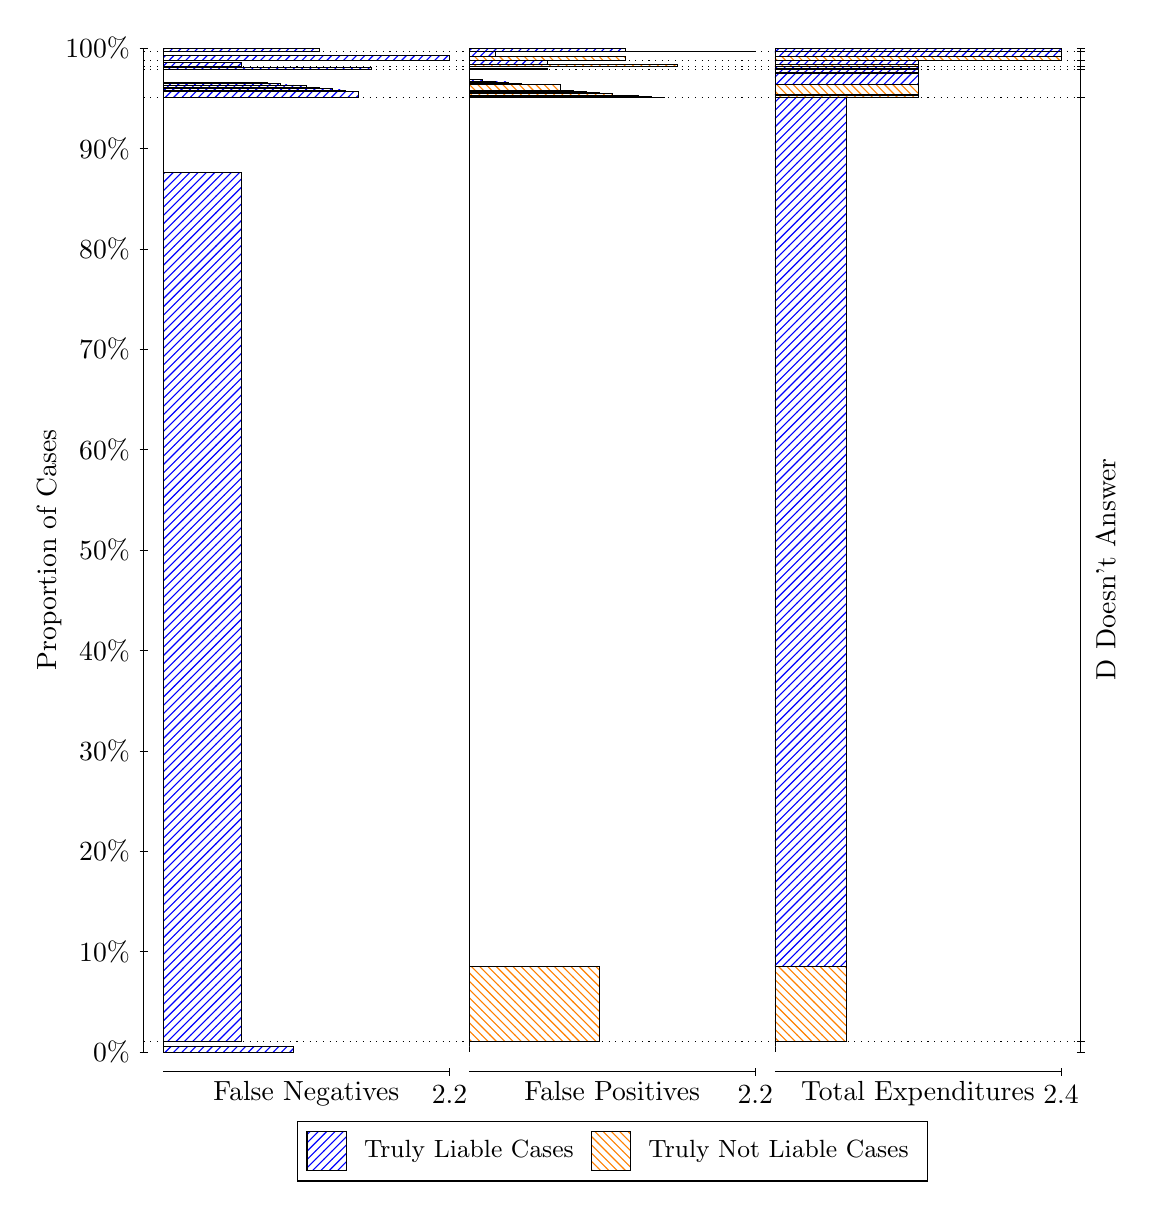
\begin{tikzpicture}
\draw[black, very thin] (1.5,1.75) -- (1.5,14.5);
\node[rotate=90, anchor=center] at (0.3, 8.125) {Proportion of Cases};
\draw[black, very thin] (1.45,1.75) -- (1.55,1.75);
\node[anchor=east] at (1.45, 1.75) {0\%};
\draw[black, very thin] (1.45,3.025) -- (1.55,3.025);
\node[anchor=east] at (1.45, 3.025) {10\%};
\draw[black, very thin] (1.45,4.3) -- (1.55,4.3);
\node[anchor=east] at (1.45, 4.3) {20\%};
\draw[black, very thin] (1.45,5.575) -- (1.55,5.575);
\node[anchor=east] at (1.45, 5.575) {30\%};
\draw[black, very thin] (1.45,6.85) -- (1.55,6.85);
\node[anchor=east] at (1.45, 6.85) {40\%};
\draw[black, very thin] (1.45,8.125) -- (1.55,8.125);
\node[anchor=east] at (1.45, 8.125) {50\%};
\draw[black, very thin] (1.45,9.4) -- (1.55,9.4);
\node[anchor=east] at (1.45, 9.4) {60\%};
\draw[black, very thin] (1.45,10.675) -- (1.55,10.675);
\node[anchor=east] at (1.45, 10.675) {70\%};
\draw[black, very thin] (1.45,11.95) -- (1.55,11.95);
\node[anchor=east] at (1.45, 11.95) {80\%};
\draw[black, very thin] (1.45,13.225) -- (1.55,13.225);
\node[anchor=east] at (1.45, 13.225) {90\%};
\draw[black, very thin] (1.45,14.5) -- (1.55,14.5);
\node[anchor=east] at (1.45, 14.5) {100\%};

\draw[black, very thin] (13.4,1.75) -- (13.4,14.5);
\draw[black, very thin] (13.35,1.75) -- (13.45,1.75);
\node[anchor=west] at (13.35, 1.75) {};
\draw[black, very thin] (13.35,1.887) -- (13.45,1.887);
\node[anchor=west] at (13.35, 1.887) {};
\draw[black, very thin] (13.35,13.874) -- (13.45,13.874);
\node[anchor=west] at (13.35, 13.874) {};
\draw[black, very thin] (13.35,14.228) -- (13.45,14.228);
\node[anchor=west] at (13.35, 14.228) {};
\draw[black, very thin] (13.35,14.267) -- (13.45,14.267);
\node[anchor=west] at (13.35, 14.267) {};
\draw[black, very thin] (13.35,14.343) -- (13.45,14.343);
\node[anchor=west] at (13.35, 14.343) {};
\draw[black, very thin] (13.35,14.456) -- (13.45,14.456);
\node[anchor=west] at (13.35, 14.456) {};
\draw[black, very thin] (13.35,14.5) -- (13.45,14.5);
\node[anchor=west] at (13.35, 14.5) {};

\draw[black, very thin, pattern color=blue, pattern=north east lines] (1.75,1.75) rectangle (3.4015,1.8204);
\draw[black, very thin, pattern color=orange, pattern=north west lines] (1.75,1.8204) rectangle (1.75,1.887);
\draw[black, very thin, pattern color=blue, pattern=north east lines] (1.75,1.887) rectangle (2.7409,12.925);
\draw[black, very thin, pattern color=orange, pattern=north west lines] (1.75,12.925) rectangle (1.75,13.874);
\draw[black, very thin, pattern color=blue, pattern=north east lines] (1.75,13.874) rectangle (4.2273,13.953);
\draw[black, very thin, pattern color=blue, pattern=north east lines] (1.75,13.953) rectangle (4.0621,13.969);
\draw[black, very thin, pattern color=blue, pattern=north east lines] (1.75,13.969) rectangle (3.897,13.986);
\draw[black, very thin, pattern color=blue, pattern=north east lines] (1.75,13.986) rectangle (3.7318,14.004);
\draw[black, very thin, pattern color=blue, pattern=north east lines] (1.75,14.004) rectangle (3.5667,14.026);
\draw[black, very thin, pattern color=blue, pattern=north east lines] (1.75,14.026) rectangle (3.4015,14.033);
\draw[black, very thin, pattern color=blue, pattern=north east lines] (1.75,14.033) rectangle (3.2364,14.05);
\draw[black, very thin, pattern color=blue, pattern=north east lines] (1.75,14.05) rectangle (3.0712,14.062);
\draw[black, very thin, pattern color=blue, pattern=north east lines] (1.75,14.062) rectangle (2.9061,14.067);
\draw[black, very thin, pattern color=orange, pattern=north west lines] (1.75,14.067) rectangle (1.75,14.228);
\draw[black, very thin, pattern color=blue, pattern=north east lines] (1.75,14.228) rectangle (4.3924,14.25);
\draw[black, very thin, pattern color=orange, pattern=north west lines] (1.75,14.25) rectangle (1.75,14.267);
\draw[black, very thin, pattern color=blue, pattern=north east lines] (1.75,14.267) rectangle (2.7409,14.32);
\draw[black, very thin, pattern color=orange, pattern=north west lines] (1.75,14.32) rectangle (1.75,14.343);
\draw[black, very thin, pattern color=blue, pattern=north east lines] (1.75,14.343) rectangle (5.3833,14.403);
\draw[black, very thin, pattern color=orange, pattern=north west lines] (1.75,14.403) rectangle (1.75,14.456);
\draw[black, very thin, pattern color=blue, pattern=north east lines] (1.75,14.456) rectangle (3.7318,14.494);
\draw[black, very thin, pattern color=orange, pattern=north west lines] (1.75,14.494) rectangle (1.75,14.5);
\draw[black, very thin, pattern color=orange, pattern=north west lines] (5.6333,1.75) rectangle (5.6333,1.8166);
\draw[black, very thin, pattern color=blue, pattern=north east lines] (5.6333,1.8166) rectangle (5.6333,1.887);
\draw[black, very thin, pattern color=orange, pattern=north west lines] (5.6333,1.887) rectangle (7.2848,2.8364);
\draw[black, very thin, pattern color=blue, pattern=north east lines] (5.6333,2.8364) rectangle (5.6333,13.874);
\draw[black, very thin, pattern color=orange, pattern=north west lines] (5.6333,13.874) rectangle (8.1106,13.876);
\draw[black, very thin, pattern color=orange, pattern=north west lines] (5.6333,13.876) rectangle (7.9455,13.883);
\draw[black, very thin, pattern color=orange, pattern=north west lines] (5.6333,13.883) rectangle (7.7803,13.894);
\draw[black, very thin, pattern color=orange, pattern=north west lines] (5.6333,13.894) rectangle (7.6152,13.9);
\draw[black, very thin, pattern color=orange, pattern=north west lines] (5.6333,13.9) rectangle (7.45,13.92);
\draw[black, very thin, pattern color=orange, pattern=north west lines] (5.6333,13.92) rectangle (7.2848,13.935);
\draw[black, very thin, pattern color=orange, pattern=north west lines] (5.6333,13.935) rectangle (7.1197,13.951);
\draw[black, very thin, pattern color=orange, pattern=north west lines] (5.6333,13.951) rectangle (6.9545,13.966);
\draw[black, very thin, pattern color=orange, pattern=north west lines] (5.6333,13.966) rectangle (6.7894,14.035);
\draw[black, very thin, pattern color=blue, pattern=north east lines] (5.6333,14.035) rectangle (6.4591,14.04);
\draw[black, very thin, pattern color=blue, pattern=north east lines] (5.6333,14.04) rectangle (6.2939,14.052);
\draw[black, very thin, pattern color=blue, pattern=north east lines] (5.6333,14.052) rectangle (6.1288,14.069);
\draw[black, very thin, pattern color=blue, pattern=north east lines] (5.6333,14.069) rectangle (5.9636,14.076);
\draw[black, very thin, pattern color=blue, pattern=north east lines] (5.6333,14.076) rectangle (5.7985,14.098);
\draw[black, very thin, pattern color=blue, pattern=north east lines] (5.6333,14.098) rectangle (5.6333,14.228);
\draw[black, very thin, pattern color=orange, pattern=north west lines] (5.6333,14.228) rectangle (6.6242,14.245);
\draw[black, very thin, pattern color=blue, pattern=north east lines] (5.6333,14.245) rectangle (5.6333,14.267);
\draw[black, very thin, pattern color=orange, pattern=north west lines] (5.6333,14.267) rectangle (8.2758,14.289);
\draw[black, very thin, pattern color=blue, pattern=north east lines] (5.6333,14.289) rectangle (6.6242,14.343);
\draw[black, very thin, pattern color=orange, pattern=north west lines] (5.6333,14.343) rectangle (7.6152,14.395);
\draw[black, very thin, pattern color=blue, pattern=north east lines] (5.6333,14.395) rectangle (5.9636,14.456);
\draw[black, very thin, pattern color=orange, pattern=north west lines] (5.6333,14.456) rectangle (9.2667,14.462);
\draw[black, very thin, pattern color=blue, pattern=north east lines] (5.6333,14.462) rectangle (7.6152,14.5);
\draw[black, very thin, pattern color=orange, pattern=north west lines] (9.5167,1.75) rectangle (9.5167,1.8166);
\draw[black, very thin, pattern color=blue, pattern=north east lines] (9.5167,1.8166) rectangle (9.5167,1.887);
\draw[black, very thin, pattern color=orange, pattern=north west lines] (9.5167,1.887) rectangle (10.425,2.8364);
\draw[black, very thin, pattern color=blue, pattern=north east lines] (9.5167,2.8364) rectangle (10.425,13.874);
\draw[black, very thin, pattern color=orange, pattern=north west lines] (9.5167,13.874) rectangle (11.333,13.894);
\draw[black, very thin, pattern color=blue, pattern=north east lines] (9.5167,13.894) rectangle (11.333,13.916);
\draw[black, very thin, pattern color=orange, pattern=north west lines] (9.5167,13.916) rectangle (11.333,14.038);
\draw[black, very thin, pattern color=blue, pattern=north east lines] (9.5167,14.038) rectangle (11.333,14.18);
\draw[black, very thin, pattern color=orange, pattern=north west lines] (9.5167,14.18) rectangle (11.333,14.198);
\draw[black, very thin, pattern color=blue, pattern=north east lines] (9.5167,14.198) rectangle (11.333,14.228);
\draw[black, very thin, pattern color=orange, pattern=north west lines] (9.5167,14.228) rectangle (11.333,14.245);
\draw[black, very thin, pattern color=blue, pattern=north east lines] (9.5167,14.245) rectangle (11.333,14.267);
\draw[black, very thin, pattern color=orange, pattern=north west lines] (9.5167,14.267) rectangle (11.333,14.289);
\draw[black, very thin, pattern color=blue, pattern=north east lines] (9.5167,14.289) rectangle (11.333,14.343);
\draw[black, very thin, pattern color=orange, pattern=north west lines] (9.5167,14.343) rectangle (13.15,14.395);
\draw[black, very thin, pattern color=blue, pattern=north east lines] (9.5167,14.395) rectangle (13.15,14.456);
\draw[black, very thin, pattern color=orange, pattern=north west lines] (9.5167,14.456) rectangle (13.15,14.462);
\draw[black, very thin, pattern color=blue, pattern=north east lines] (9.5167,14.462) rectangle (13.15,14.5);
\draw[black, dotted] (1.5,1.887) -- (13.4,1.887);
\draw[black, dotted] (1.5,13.874) -- (13.4,13.874);
\draw[black, dotted] (1.5,14.228) -- (13.4,14.228);
\draw[black, dotted] (1.5,14.267) -- (13.4,14.267);
\draw[black, dotted] (1.5,14.343) -- (13.4,14.343);
\draw[black, dotted] (1.5,14.456) -- (13.4,14.456);
\draw[black, very thin] (1.75,1.5) -- (5.3833,1.5);
\node[anchor=north] at (3.5667, 1.5) {False Negatives};
\draw[black, very thin] (5.3833,1.45) -- (5.3833,1.55);
\node[anchor=north] at (5.3833, 1.45) {2.2};

\draw[black, very thin] (5.6333,1.5) -- (9.2667,1.5);
\node[anchor=north] at (7.45, 1.5) {False Positives};
\draw[black, very thin] (9.2667,1.45) -- (9.2667,1.55);
\node[anchor=north] at (9.2667, 1.45) {2.2};

\draw[black, very thin] (9.5167,1.5) -- (13.15,1.5);
\node[anchor=north] at (11.333, 1.5) {Total Expenditures};
\draw[black, very thin] (13.15,1.45) -- (13.15,1.55);
\node[anchor=north] at (13.15, 1.45) {2.4};


\node[black, centered, rotate=90] at (13.72, 7.8804) {D Doesn't Answer};






\draw (7.449999999999999,1.5) node[draw=none] (baseCoordinate) {};
\begin{scope}[align=center]
        \matrix[scale=0.5, draw=black, below=0.5cm of baseCoordinate, nodes={draw}, column sep=0.1cm]{
            \node[rectangle, draw, minimum width=0.5cm, minimum height=0.5cm, pattern=north east lines, pattern color=blue] {}; &
            \node[draw=none, font=\small] (B) {Truly Liable Cases}; &
            \node[rectangle, draw, minimum width=0.5cm, minimum height=0.5cm, pattern=north west lines, pattern color=orange] {}; &
            \node[draw=none, font=\small] (B) {Truly Not Liable Cases}; \\
            };
\end{scope}

\end{tikzpicture}
\end{document}